\documentclass[11pt,a4paper]{article}

% ---------------------------------------------------------------------------
% Reactant-bimolecular mass-action instability without D-unstable cores.
%
% Author metadata: set the three macros below before submission.
% ---------------------------------------------------------------------------
\newcommand{\PaperAuthor}{}
\newcommand{\PaperAffiliation}{}
\newcommand{\PaperDate}{September 2026}

\usepackage[T1]{fontenc}
\usepackage[utf8]{inputenc}
\usepackage{lmodern}
\usepackage{microtype}
\usepackage[a4paper,margin=1.05in]{geometry}
\usepackage{amsmath,amssymb,amsthm,mathtools}
\usepackage{booktabs}
\usepackage{array}
\usepackage{enumitem}
\usepackage{graphicx}
\usepackage{xcolor}
\usepackage[obeyspaces,spaces]{url}
\usepackage[colorlinks=true,linkcolor=blue!55!black,citecolor=blue!55!black,urlcolor=blue!55!black]{hyperref}

\setlist{itemsep=2pt,topsep=3pt}
\setlength{\emergencystretch}{1.5em}

\theoremstyle{plain}
\newtheorem{theorem}{Theorem}[section]
\newtheorem{proposition}[theorem]{Proposition}
\newtheorem{lemma}[theorem]{Lemma}
\newtheorem{corollary}[theorem]{Corollary}
\theoremstyle{definition}
\newtheorem{definition}[theorem]{Definition}
\newtheorem{example}[theorem]{Example}
\newtheorem{question}[theorem]{Question}
\theoremstyle{remark}
\newtheorem{remark}[theorem]{Remark}

\newcommand{\R}{\mathbb{R}}
\newcommand{\Q}{\mathbb{Q}}
\newcommand{\N}{\mathbb{N}}
\newcommand{\Z}{\mathbb{Z}}
\newcommand{\C}{\mathbb{C}}
\newcommand{\diag}{\operatorname{diag}}
\newcommand{\supp}{\operatorname{supp}}
\newcommand{\Real}{\operatorname{Re}}
\newcommand{\Imag}{\operatorname{Im}}
\newcommand{\spec}{\operatorname{spec}}
\newcommand{\DN}{\mathcal{N}_D}
\newcommand{\xs}{x^{*}}
\newcommand{\vs}{v^{*}}
\newcommand{\Ract}{\mathrm{R2}}
\newcommand{\Rcf}{\mathrm{R2\text{-}CF}}
\newcommand{\Rpp}{\mathrm{R2P2}}
\DeclareUrlCommand\lean{\urlstyle{tt}}

\title{Reactant-bimolecular mass-action instability\\ without D-unstable cores}
\author{\PaperAuthor\\ \PaperAffiliation}
\date{\PaperDate}

\begin{document}
\maketitle

\begin{abstract}
A child selection of a reaction network assigns to each species in a subset a distinct reaction consuming it; the corresponding square submatrix of the stoichiometric matrix is D-unstable if some positive diagonal column scaling gives it an eigenvalue with positive real part. Vassena and Stadler proved that a minimal such submatrix, a D-unstable core, forces an unstable positive equilibrium under every parameter-rich kinetics, and conjectured the converse. The converse is known to fail for parameter-rich kinetics and, through catalytic padding with large kinetic orders, for classical mass action; the question whether it fails when every reaction consumes at most two molecules had remained open. We answer it in the negative. We give a four-species, six-reaction mass-action network in which every reactant complex has at most two molecules and no species occurs on both sides of any reaction, with integer rate constants and the positive equilibrium $(1,1,1,1/100)$, whose Jacobian has an eigenvalue with real part in $[2,4]$, although every one of its $25$ child-selection matrices is D-nonunstable under every positive diagonal scaling. The instability proof is an exact shifted Routh--Hurwitz construction; the child proof reduces all children to four maximal selections by a principal-restriction lemma and certifies each by positivity of the third Hurwitz determinant as a polynomial in the scalings. We then parameterize the complete positive stationary-flux cone of the network, $v=s(T,4,T,1,T-1,2)$ with $T>1$, and prove that along the concentration family $\xs=(1,1,1,1/L)$ the equilibrium is unstable for $T=100$ and every $L\ge100$, while $(T,L)=(2,1)$ is an exactly certified stable operating point of the same network with the same children. The instability persists under all sufficiently small independent perturbations of the six rate constants, and under a feed-and-dilution completion with dilution rate below $2$. Reactant molecularity two is sharp: every positive equilibrium of a mass-action network whose reactions consume at most one molecule is Hurwitz-nonunstable, and four species is the least possible number. The network admits no positive mass vector, so it is a kinetic, not an atom-resolved, counterexample; the two-sided bimolecular question remains open. The source-level existence theorem and the negation of universal reactant-bimolecular core necessity are verified in Lean~4 with Mathlib.
\end{abstract}

\noindent\textbf{Keywords.} chemical reaction networks; mass-action kinetics; unstable cores; child selections; D-stability; bimolecular reactions; Routh--Hurwitz criterion; formal verification.

\medskip
\noindent\textbf{MSC 2020.} 80A30, 92C42, 34D20, 15A18, 15B48, 68V20.

\section{Introduction}\label{sec:intro}

A recurring aim of chemical reaction network theory is to decide dynamical questions from the network structure alone, because rate constants are rarely known~\cite{Feinberg2019,Clarke1980}. For the question whether some positive equilibrium can be linearly unstable, Vassena and Stadler~\cite{VassenaStadler2024} gave a clean structural sufficient condition. A \emph{child selection} assigns to each species of a subset a distinct reaction in which that species is a reactant; the selected columns of the stoichiometric matrix $S$, restricted to the selected rows, form a square \emph{child-selection matrix}. If some child-selection matrix is \emph{D-unstable}, that is, acquires an eigenvalue with positive real part after multiplication by some positive diagonal matrix, then for every \emph{parameter-rich} kinetics the network admits an unstable positive equilibrium. A minimal such child selection is a \emph{D-unstable core}. The authors conjectured the converse~\cite[Conj.~17]{VassenaStadler2024}: a network without D-unstable cores admits no instability.

The conjecture is false as stated: an exact four-species, five-reaction parameter-rich counterexample is given in the companion manuscript~\cite{ParameterRich2026}. Classical mass action is far more rigid than parameter-rich kinetics, since all reaction sensitivities are tied to the same fluxes and concentrations, and one may hope that this rigidity rescues localization. The second companion manuscript~\cite{KineticOrder2026} shows that it does not: any prescribed admissible reactivity can be realized by ordinary mass action after \emph{catalytic padding}, which adds the same nonnegative integer matrix to both sides of every reaction and thereby leaves every child-selection matrix unchanged. The counterexamples obtained in this way, however, use reactant complexes with tens, hundreds or thousands of molecules. Reactions that consume at most two molecules are the physically elementary ones, and the following question was left open there~\cite[Question~8.1]{KineticOrder2026}: does D-unstable-core localization hold for classical mass-action networks in which every reaction has at most two reactant molecules, or in which no species occurs on both sides of a reaction?

This paper answers both parts of that question in the negative, with a single explicit network.

\subsection{Main results}

Write $\Ract$ for the class of finite mass-action networks in which every reaction consumes at most two molecules in total (\emph{reactant-bimolecular}), and $\Rcf$ for the subclass in which additionally no species is both a reactant and a product of the same reaction (\emph{catalyst-free}). Inflows $\varnothing\to X$ are allowed in both classes. A matrix $C$ is \emph{D-nonunstable}, written $C\in\DN$, if for every positive diagonal $D$ every eigenvalue of $CD$ has real part at most zero. This boundary-permitting notion, not strict D-stability, is the one the conjecture negates; the distinction matters here because four of the $25$ child matrices below are singular.

\begin{theorem}[Theorem~\ref{thm:main}]\label{thm:A}
There is a mass-action network with four species and six reactions in $\Rcf$, with positive integer rate constants and the positive equilibrium $\xs=(1,1,1,1/100)$, whose Jacobian at $\xs$ has an eigenvalue with real part in the interval $[2,4]$, while every one of its $25$ child-selection matrices is D-nonunstable. Consequently the network has no D-unstable core, and universal D-core necessity is false in the classes $\Ract$ and $\Rcf$.
\end{theorem}

The network is
\[
A+D\to2C,\qquad B+C\to\varnothing,\qquad 2C\to D,\qquad 2D\to A+4B+4C,\qquad \varnothing\to A,\qquad\varnothing\to D,
\]
with rate constants $(10000,4,100,10000,99,2)$. Its characteristic polynomial at $\xs$ is
\[
p(z)=z^4+10908z^3+185600z^2+1280000z+64000000,
\]
whose third Hurwitz determinant is negative although all coefficients are positive: the instability is of complex-pair type, as it must be, since a positive real eigenvalue would force a D-unstable child~\cite{ParameterRich2026}.

The example is not an isolated point. The second group of results describes the operating conditions of the same network.

\begin{theorem}[Propositions~\ref{prop:cone}--\ref{prop:stable}]\label{thm:B}
The positive stationary fluxes of the network are exactly $v=s(T,4,T,1,T-1,2)$ with $s>0$ and $T>1$, and every such flux is realized at every positive concentration vector by unique positive rate constants. Along the family $\xs=(1,1,1,1/L)$, the characteristic polynomial of the equilibrium Jacobian has the coefficients
\[
a_1=(T+4)L+5T+8,\quad a_2=(14T+32)L+4T(T+6),\quad a_3=112TL+16T^2,\quad a_4=64T^2L,
\]
up to the time scale $s$. For $T=100$ and every $L\ge100$ the equilibrium is unstable; for $(T,L)=(2,1)$, that is, for rate constants $(2,4,2,1,1,2)$ and the equilibrium $(1,1,1,1)$, it is strictly Hurwitz stable. For every $T>T_*=(41+\sqrt{2577})/4$ the equilibrium is unstable for all sufficiently large $L$, and for $1<T<T_*$ it is Hurwitz-nonunstable for all sufficiently large $L$.
\end{theorem}

The stable and unstable operating points have the same stoichiometric matrix, the same reactant incidences and the same $25$ child certificates. What the child criterion cannot see is the simultaneous, flux-constrained combination of reaction sensitivities in the whole Jacobian; Section~\ref{sec:mechanism} makes this precise through a fast-$D$ Schur reduction whose Hurwitz determinant changes sign at $T_*$.

\begin{theorem}[Theorems~\ref{thm:robust} and~\ref{thm:dilution}]\label{thm:C}
The instability persists under all sufficiently small independent perturbations of the six rate constants, with a nearby positive equilibrium. If first-order losses $X\to\varnothing$ at a common rate $\delta$ are added for all four species and the inflows are adjusted to $(99+\delta,\delta,\delta,2+\delta/100)$, the point $\xs$ remains an equilibrium of the resulting twelve-reaction network, the network remains in $\Rcf$ with no D-unstable core, and the equilibrium remains unstable for every $0<\delta<2$.
\end{theorem}

\begin{theorem}[Theorem~\ref{thm:R1} and Proposition~\ref{prop:species}]\label{thm:D}
If every reaction of a finite mass-action network consumes at most one molecule, then every positive equilibrium is Hurwitz-nonunstable, for all positive rate constants. Hence reactant molecularity two is the least for which an unstable equilibrium without D-unstable cores can occur. In any kinetics with admissible reactivity, and in particular in mass action, a network with at most three species whose children are all D-nonunstable has a D-nonunstable Jacobian; hence four species is the least possible number.
\end{theorem}

\subsection{What is not claimed}

The largest product complex, $A+4B+4C$, has nine molecules. The example therefore does not decide whether localization holds when both reactant and product molecularities are bounded by two (the class $\Rpp$); that remains open. The network admits no positive mass vector (Proposition~\ref{prop:mass}), so it is a counterexample about mass-action kinetics on abstract species, not an atom-resolved chemical mechanism. An unstable complex eigenpair is not a Hopf bifurcation theorem, a periodic orbit, or a persistence statement; Figure~\ref{fig:local} is a numerical illustration only. Six reactions and product molecularity nine are not claimed to be minimal. This is also not the first mass-action counterexample: that is~\cite{KineticOrder2026}. The contribution is that the low-molecularity restriction, which is the physically natural one, does not restore localization.

\subsection{Method and organization}

The instability proof avoids numerical eigenvalues: for the shifted polynomial $p(z+t)$ the third Hurwitz determinant $H(t)$ changes sign on $[2,4]$, and a zero of $H$ produces an explicit purely imaginary root of $p(z+t)$, hence a root of $p$ with real part $t$ (Proposition~\ref{prop:root}). The child proof uses one scalar lemma, positivity of the third Hurwitz determinant of a quartic with nonnegative coefficients excludes right-half-plane roots (Lemma~\ref{lem:quartic}), together with a principal-restriction lemma (Lemma~\ref{lem:restriction}) that reduces the $25$ children to four maximal ones. The Lean development takes the more direct route of checking all $25$ padded children individually; the two routes are logically independent.

Section~\ref{sec:setting} fixes definitions and the refuted implication. Section~\ref{sec:witness} presents the network and proves instability. Section~\ref{sec:spectral} collects the spectral lemmas. Section~\ref{sec:children} proves that every child is D-nonunstable and assembles Theorem~\ref{thm:main}. Section~\ref{sec:family} parameterizes the operating conditions and proves Theorem~\ref{thm:B}. Section~\ref{sec:robust} proves rate-space robustness and the feed-and-dilution extension. Section~\ref{sec:sharp} proves sharpness of the reactant order and species minimality. Section~\ref{sec:scope} discusses mass balance, units, a local numerical illustration, and the use of the network as a benchmark. Section~\ref{sec:formal} documents the formal verification and separates formally verified from conventionally proved statements. Section~\ref{sec:open} lists open problems.

\subsection{Related work}

Child selections and the Cauchy--Binet expansion of characteristic coefficients underlie a line of structural bifurcation results by Vassena~\cite{Vassena2023SaddleNode,Vassena2023Symbolic}; the D-unstable-core theorem and conjecture are in~\cite{VassenaStadler2024}. D-stability and its relatives originate in economics~\cite{ArrowMcManus1958,Johnson1974} and are surveyed in~\cite{Cross1978,Hershkowitz1992,Kushel2019}. The classical route from network structure to Routh--Hurwitz conditions goes back to Clarke~\cite{Clarke1980}; graph-theoretic approaches to oscillatory instabilities include~\cite{MinchevaRoussel2007,AngeliBanajiPantea2014}. Small bimolecular networks with Andronov--Hopf bifurcations were classified by Banaji and Boros~\cite{BanajiBoros2023}, and Banaji showed that splitting reactions preserves nondegenerate behaviours~\cite{Banaji2022Splitting}; Wilhelm's smallest bistable system~\cite{Wilhelm2009} is the classical minimality result of this kind. None of these supplies the all-child spectral exclusion required here, which is a statement about the entire lattice of child selections rather than about one bifurcation. The autocatalytic cores of~\cite{BlokhuisLacosteNghe2020} and the RAF sets of~\cite{HordijkSteel2004} concern structural self-sustainment; the present result separates that layer from dynamic stability (Section~\ref{sec:benchmark}).

\section{Setting and the refuted implication}\label{sec:setting}

\subsection{Sources and mass action}

Species are indexed by $\{0,\dots,n-1\}$ and reactions by $\{0,\dots,m-1\}$, matching the formal development. A \emph{source} is a pair $(Y,P)$ of matrices in $\N_0^{n\times m}$, the reactant and product matrices; $S=P-Y\in\Z^{n\times m}$ is the stoichiometric matrix. Reaction $j$ consumes the complex $\sum_iY_{ij}X_i$ and produces $\sum_iP_{ij}X_i$. The \emph{reactant molecularity} of reaction $j$ is $\sum_iY_{ij}$; the source is in $\Ract$ if all reactant molecularities are at most two, and it is \emph{catalyst-free} if $Y_{ij}P_{ij}=0$ for all $i,j$. A reaction with $Y_{\cdot j}=0$ is an \emph{inflow}. Species $i$ is a \emph{reactant} of reaction $j$ if $Y_{ij}>0$.

Ordinary mass action with rate constants $k\in\R_{>0}^m$ is the vector field
\begin{equation}\label{eq:mass}
\dot x=F(x)=S\,v(x),\qquad v_j(x)=k_j\prod_{i}x_i^{Y_{ij}},\qquad x\in\R_{>0}^n .
\end{equation}
For a homodimerization $2X\to\cdots$ the deterministic event rate is $kx^2$ and the factor $2$ in the consumption is supplied by $S$. A \emph{positive equilibrium} is $\xs\in\R^n_{>0}$ with $F(\xs)=0$; its \emph{flux} is $\vs=v(\xs)\in\R^m_{>0}$, and $S\vs=0$. Differentiating~\eqref{eq:mass} gives the derivative identity
\begin{equation}\label{eq:J}
J=DF(\xs)=S\,R,\qquad R=\diag(\vs)\,Y^{\mathsf T}\diag(\xs)^{-1},\qquad R_{ji}=\frac{Y_{ij}v^*_j}{x^*_i}.
\end{equation}
The \emph{reactivity} $R\in\R^{m\times n}_{\ge0}$ is positive exactly on the reactant incidences $Y_{ij}>0$. Conversely, for every positive $x$ and every positive $v$ with $Sv=0$ the rate constants $k_j=v_j/\prod_ix_i^{Y_{ij}}$ are positive and make $x$ an equilibrium with flux $v$; we call this \emph{rate reconstruction}. Parameter-rich kinetics in the sense of~\cite{VassenaStadler2024} allow every reactivity positive exactly on the reactant incidences; mass-action reactivities are the subfamily tied to $(\vs,\xs)$ by~\eqref{eq:J}.

\subsection{Children, D-noninstability, cores}

\begin{definition}[Child selection]\label{def:child}
A \emph{child selection} of the source $(Y,P)$ is a subset $I$ of species together with an injective map $f\colon I\to\{0,\dots,m-1\}$ with $Y_{i,f(i)}>0$ for all $i\in I$. Its \emph{child matrix} is the square matrix
\[
C_f=\bigl(S_{i,f(j)}\bigr)_{i,j\in I}\in\Z^{I\times I},
\]
with columns indexed by the species to which the reactions are assigned. The empty selection has the empty matrix.
\end{definition}

\begin{definition}[Spectral notions]\label{def:spectral}
Let $C$ be a real square matrix.
\begin{enumerate}[label=(\alph*)]
\item $C$ is \emph{Hurwitz-unstable} if it has an eigenvalue with strictly positive real part, and \emph{Hurwitz-nonunstable} otherwise.
\item $C$ is \emph{D-unstable} if $CD$ is Hurwitz-unstable for some positive diagonal matrix $D$.
\item $C$ is \emph{D-nonunstable}, $C\in\DN$, if $CD$ is Hurwitz-nonunstable for every positive diagonal $D$.
\item $C$ is \emph{D-stable} if every eigenvalue of $CD$ has strictly negative real part for every positive diagonal $D$.
\end{enumerate}
\end{definition}

D-stability implies D-noninstability, not conversely: (c) permits zero and purely imaginary eigenvalues, (d) excludes them. The conjecture of~\cite{VassenaStadler2024} and its mass-action analogue are statements about (b) and its negation (c). A \emph{D-unstable core} is a D-unstable child selection that is minimal under principal restriction, that is, under passing to a subset $I'\subseteq I$ with the same assignment. Since every D-unstable child contains a D-unstable core, a source has no D-unstable core if and only if every child matrix belongs to $\DN$.

\subsection{The implication under test}

The theorem of~\cite{VassenaStadler2024} states that a D-unstable core forces an unstable positive equilibrium under every parameter-rich kinetics. The refuted conjecture is its converse. Restricted to mass action on the class $\Ract$ it reads as follows.

\begin{quote}
\textbf{(N$_{\Ract}$)} For every source $(Y,P)$ in $\Ract$, every positive rate vector $k$ and every positive equilibrium $\xs$ of~\eqref{eq:mass}: if $DF(\xs)$ is Hurwitz-unstable, then $(Y,P)$ has a D-unstable core.
\end{quote}

Statement (N$_{\Rcf}$) is the same with $\Rcf$ in place of $\Ract$. Both are weaker than the parameter-rich conjecture and weaker than the unrestricted mass-action statement refuted in~\cite{KineticOrder2026}, because the kinetic orders in those counterexamples are large. Table~\ref{tab:classes} summarizes the landscape.

\begin{table}[ht]
\centering\footnotesize
\begin{tabular}{@{}lll@{}}
\toprule
Kinetic class & D-core necessity & Reference\\
\midrule
parameter-rich kinetics & false & \cite{ParameterRich2026}\\
mass action, unbounded kinetic order & false & \cite{KineticOrder2026}\\
mass action, at most one reactant molecule & true (no instability at all) & Theorem~\ref{thm:R1}\\
mass action, at most two reactant molecules ($\Ract$) & false & Theorem~\ref{thm:main}\\
$\Ract$ and catalyst-free ($\Rcf$) & false & Theorem~\ref{thm:main}\\
at most two reactant and two product molecules ($\Rpp$) & open & Section~\ref{sec:open}\\
at most three species, any admissible reactivity & true & Proposition~\ref{prop:species}\\
\bottomrule
\end{tabular}
\caption{Status of D-unstable-core necessity by kinetic class.}
\label{tab:classes}
\end{table}

\section{The network and its unstable equilibrium}\label{sec:witness}

\subsection{The source}

Species are $A,B,C,D$ (indices $0,1,2,3$) and reactions $r_0,\dots,r_5$. The empty complex denotes exchange with the environment.

\begin{table}[ht]
\centering\small
\begin{tabular}{@{}clcccl@{}}
\toprule
& Reaction & $\sum_iY_{ij}$ & $\sum_iP_{ij}$ & $k_j$ & Event rate\\
\midrule
$r_0$ & $A+D\to2C$ & 2 & 2 & $10000$ & $10000\,x_Ax_D$\\
$r_1$ & $B+C\to\varnothing$ & 2 & 0 & $4$ & $4\,x_Bx_C$\\
$r_2$ & $2C\to D$ & 2 & 1 & $100$ & $100\,x_C^2$\\
$r_3$ & $2D\to A+4B+4C$ & 2 & 9 & $10000$ & $10000\,x_D^2$\\
$r_4$ & $\varnothing\to A$ & 0 & 1 & $99$ & $99$\\
$r_5$ & $\varnothing\to D$ & 0 & 1 & $2$ & $2$\\
\bottomrule
\end{tabular}
\caption{The reactant-bimolecular, catalyst-free source $\mathcal E$ with its rate constants.}
\label{tab:source}
\end{table}

The literal matrices are
\begin{equation}\label{eq:source}
Y=\begin{pmatrix}
1&0&0&0&0&0\\0&1&0&0&0&0\\0&1&2&0&0&0\\1&0&0&2&0&0
\end{pmatrix},\qquad
S=P-Y=\begin{pmatrix}
-1&0&0&1&1&0\\0&-1&0&4&0&0\\2&-1&-2&4&0&0\\-1&0&1&-2&0&1
\end{pmatrix}.
\end{equation}
Every column of $Y$ sums to at most two and $Y_{ij}P_{ij}=0$ throughout, so $\mathcal E\in\Rcf$. The maximal product molecularity is nine, attained by $r_3$.

\subsection{Equilibrium and Jacobian}

At
\begin{equation}\label{eq:state}
\xs=\bigl(1,1,1,\tfrac1{100}\bigr)^{\mathsf T},\qquad
\vs=v(\xs)=(100,4,100,1,99,2)^{\mathsf T},
\end{equation}
the six event rates evaluate exactly to the displayed flux, and $S\vs=0$ row by row: $-100+1+99=0$, $-4+4=0$, $200-4-200+4=0$, $-100+100-2+2=0$. Thus $\xs$ is a positive equilibrium. Formula~\eqref{eq:J} gives
\begin{equation}\label{eq:jac}
J=\begin{pmatrix}
-100&0&0&-9800\\
0&-4&-4&800\\
200&-4&-404&20800\\
-100&0&200&-10400
\end{pmatrix},
\end{equation}
with characteristic polynomial
\begin{equation}\label{eq:charpoly}
p(z)=\det(zI-J)=z^4+10908z^3+185600z^2+1280000z+64000000 .
\end{equation}
These are integer determinant identities. All four coefficients are positive, $a_1a_2-a_3=2023244800>0$, and the third Hurwitz determinant is
\[
a_1a_2a_3-a_3^2-a_1^2a_4=-5025252352000000<0 .
\]

\subsection{An exact unstable root}

We prove instability without computing eigenvalues numerically.

\begin{proposition}[Exact unstable root]\label{prop:root}
The polynomial $p$ has a nonreal root $t+iw$ with $t\in[2,4]$ and $w>0$. Consequently $J$ is Hurwitz-unstable, with an eigenvalue of real part at least $2$.
\end{proposition}

\begin{proof}
For real $t$ write $p(z+t)=z^4+A(t)z^3+B(t)z^2+C(t)z+D(t)$, where
\begin{align*}
A(t)&=10908+4t,\\
B(t)&=185600+32724t+6t^2,\\
C(t)&=1280000+371200t+32724t^2+4t^3,\\
D(t)&=64000000+1280000t+185600t^2+10908t^3+t^4 .
\end{align*}
Put $H(t)=A(t)B(t)C(t)-C(t)^2-A(t)^2D(t)$. Exact substitution gives
\begin{equation}\label{eq:endpoints}
H(2)=-2133097221521408<0,\qquad H(4)=2676722101092352>0 .
\end{equation}
By continuity there is $t\in(2,4)$ with $H(t)=0$. At this $t$ the values $A(t)$ and $C(t)$ are positive, so $w=\sqrt{C(t)/A(t)}>0$ is defined and $C(t)=A(t)w^2$. Substituting into $H(t)=0$ and dividing by $A(t)$ gives $D(t)=B(t)w^2-w^4$. Therefore
\[
p(t+iw)=\bigl(w^4-B(t)w^2+D(t)\bigr)+i\bigl(C(t)w-A(t)w^3\bigr)=0 .
\]
A root of the characteristic polynomial is an eigenvalue, so $J$ has an eigenvalue with real part $t\ge2$.
\end{proof}

\begin{remark}[Root count]\label{rem:routh}
The Routh array of $p$ has first column $1$, $a_1$, $(a_1a_2-a_3)/a_1$, $(a_1a_2a_3-a_3^2-a_1^2a_4)/(a_1a_2-a_3)$, $a_4$, with signs $+,+,+,-,+$. Two sign changes give exactly two roots in the open right half-plane~\cite[Ch.~XV]{Gantmacher1959}, necessarily the conjugate pair of Proposition~\ref{prop:root}. Numerically they are $2.99974676\pm15.68952573\,i$; the other two roots are near $-23.03$ and $-10890.97$. Only the existence statement of Proposition~\ref{prop:root} is used below, and only it is formally verified.
\end{remark}

\section{Spectral lemmas}\label{sec:spectral}

Throughout, $q(z)=z^4+\alpha z^3+\beta z^2+\gamma z+\eta$ is a real monic quartic and $\Delta(q)=\alpha\beta\gamma-\gamma^2-\alpha^2\eta$ is its third Hurwitz determinant.

\begin{lemma}[Quartic exclusion]\label{lem:quartic}
Suppose $\alpha,\gamma>0$, $\beta,\eta\ge0$ and $\Delta(q)\ge0$. Then $q$ has no root in the open right half-plane.
\end{lemma}

\begin{proof}
For real $x>0$ all terms of $q(x)$ are nonnegative and $\alpha x^3>0$, so there is no positive real root. Suppose $x+iy$ is a root with $x>0$ and $y\ne0$. Then $x-iy$ is also a root, and $q$ factors over $\R$ as
\[
q(z)=(z^2-2xz+Q)(z^2+Rz+U),\qquad Q=x^2+y^2,\quad R=\alpha+2x,\quad U=\beta+2xR-Q,
\]
where comparing coefficients gives $\gamma=RQ-2xU$ and $\eta=QU$. Substituting these four expressions into $\Delta(q)$ and expanding yields the identity
\[
\Delta(q)=-2xR\bigl((Q-U)^2+\alpha\gamma\bigr).
\]
Since $x>0$, $R>0$ and $\alpha\gamma>0$, this is strictly negative, contradicting $\Delta(q)\ge0$.
\end{proof}

\begin{lemma}[Imaginary roots]\label{lem:imag}
If $i\omega$ with $\omega\ne0$ real is a root of $q$, then $\gamma=\alpha\omega^2$, $\eta=\beta\omega^2-\omega^4$, and $\Delta(q)=0$.
\end{lemma}

\begin{proof}
$q(i\omega)=(\omega^4-\beta\omega^2+\eta)+i(\gamma\omega-\alpha\omega^3)$. Both parts vanish, giving the two relations; then $\Delta(q)=\alpha\beta\cdot\alpha\omega^2-\alpha^2\omega^4-\alpha^2(\beta\omega^2-\omega^4)=0$.
\end{proof}

\begin{lemma}[Quartic instability]\label{lem:converse}
Suppose $\alpha,\beta,\gamma,\eta>0$ and $\Delta(q)<0$. Then $q$ has a root in the open right half-plane.
\end{lemma}

\begin{proof}
Zero is not a root since $\eta>0$, and nonzero imaginary roots are excluded by Lemma~\ref{lem:imag}. If no root had positive real part, all four roots would lie in the open left half-plane. Grouping conjugate pairs together and real roots in pairs gives a factorization $q(z)=(z^2+pz+q_0)(z^2+rz+t)$ with $p,q_0,r,t>0$, and expanding,
\[
\Delta(q)=pr\bigl((q_0-t)^2+(p+r)(pt+rq_0)\bigr)>0,
\]
contradicting $\Delta(q)<0$.
\end{proof}

\begin{lemma}[Principal restriction]\label{lem:restriction}
If $C\in\DN$ and $I$ is a subset of its index set, then the principal submatrix $C_I\in\DN$.
\end{lemma}

\begin{proof}
Fix a positive diagonal $D_I$ on $I$ and, for $\varepsilon>0$, let $D_\varepsilon$ be the positive diagonal matrix equal to $D_I$ on $I$ and to $\varepsilon$ on the complement. Ordering $I$ first,
\[
CD_\varepsilon\xrightarrow[\varepsilon\downarrow0]{}
\begin{pmatrix}C_ID_I&0\\ C_{I^cI}D_I&0\end{pmatrix}=:C_0 ,
\]
and $\spec(C_0)=\spec(C_ID_I)\cup\{0\}$. If $C_ID_I$ had an eigenvalue $\lambda$ with $\Real\lambda>0$, choose a closed disk around $\lambda$ inside the open right half-plane whose boundary contains no eigenvalue of $C_0$. Eigenvalues depend continuously on the matrix~\cite[App.~D]{HornJohnson2013}, so for all small $\varepsilon>0$ the matrix $CD_\varepsilon$ has an eigenvalue in that disk, contradicting $C\in\DN$. Multiple eigenvalues and singular limits cause no difficulty.
\end{proof}

\section{Every child is D-nonunstable}\label{sec:children}

\subsection{Enumeration}

Inflows have no reactants and cannot be selected. From~\eqref{eq:source}, the reactions available to each species are
\begin{equation}\label{eq:choices}
A\colon\{r_0\},\qquad B\colon\{r_1\},\qquad C\colon\{r_1,r_2\},\qquad D\colon\{r_0,r_3\}.
\end{equation}
Allowing each species to be absent gives $2\cdot2\cdot3\cdot3=36$ assignment patterns. Injectivity forbids $A\mapsto r_0$ together with $D\mapsto r_0$ ($6$ patterns) and $B\mapsto r_1$ together with $C\mapsto r_1$ ($6$ patterns, one of which is counted twice), so $11$ patterns are illegal and there are exactly $25$ child selections, including the empty one.

\begin{lemma}[Four maximal selections]\label{lem:maximal}
Every child selection is a principal restriction of one of the four selections in Table~\ref{tab:maximal}.
\end{lemma}

\begin{table}[ht]
\centering
\begin{tabular}{@{}clll@{}}
\toprule
& Species & Assigned reactions & Child matrix\\
\midrule
$M_1$ & $A,B,C,D$ & $r_0,r_1,r_2,r_3$ &
$\begin{pmatrix}-1&0&0&1\\0&-1&0&4\\2&-1&-2&4\\-1&0&1&-2\end{pmatrix}$\\[14pt]
$M_2$ & $B,C,D$ & $r_1,r_2,r_0$ &
$\begin{pmatrix}-1&0&0\\-1&-2&2\\0&1&-1\end{pmatrix}$\\[10pt]
$M_3$ & $A,C,D$ & $r_0,r_1,r_3$ &
$\begin{pmatrix}-1&0&1\\2&-1&4\\-1&0&-2\end{pmatrix}$\\[10pt]
$M_4$ & $C,D$ & $r_1,r_0$ &
$\begin{pmatrix}-1&2\\0&-1\end{pmatrix}$\\
\bottomrule
\end{tabular}
\caption{The four maximal child selections of $\mathcal E$. Rows and columns are in species order.}
\label{tab:maximal}
\end{table}

\begin{proof}
Let $(I,f)$ be a child selection. If $C\mapsto r_1$ then $B\notin I$; if $D\mapsto r_0$ then $A\notin I$. In the four cases (whether or not $C\mapsto r_1$, whether or not $D\mapsto r_0$) extend $f$ as follows: fill a missing $B$ by $r_1$ unless $C\mapsto r_1$, fill a missing $A$ by $r_0$ unless $D\mapsto r_0$, fill a missing $C$ by $r_2$, and fill a missing $D$ by $r_3$. Existing assignments are unchanged, the extension is injective, and the result is $M_1$, $M_2$, $M_3$ or $M_4$ according to the case. The original child matrix is the principal submatrix of the extension on $I$.
\end{proof}

\subsection{Certificates}

Write $a,b,c,d>0$ for the diagonal scalings of the columns belonging to $A,B,C,D$.

\begin{proposition}[Maximal children]\label{prop:maximal}
$M_1,M_2,M_3,M_4\in\DN$.
\end{proposition}

\begin{proof}
Direct expansion gives
\begin{align*}
\det\bigl(zI-M_2\diag(b,c,d)\bigr)&=z\,(z+b)\,(z+2c+d),\\
\det\bigl(zI-M_3\diag(a,c,d)\bigr)&=(z+c)\bigl(z^2+(a+2d)z+3ad\bigr),\\
\det\bigl(zI-M_4\diag(c,d)\bigr)&=(z+c)(z+d).
\end{align*}
Every root has nonpositive real part: the linear factors have negative roots, and the quadratic factor has positive coefficients. The zero eigenvalue of $M_2\diag(b,c,d)$ is permanent; $M_2$ is D-nonunstable but not D-stable.

For $M_1\diag(a,b,c,d)$ the characteristic polynomial is $z^4+A_1z^3+A_2z^2+A_3z+A_4$ with
\begin{equation}\label{eq:fullcoeff}
A_1=a+b+2c+2d,\quad
A_2=ab+2ac+3ad+2bc+2bd,\quad
A_3=2abc+3abd+4bcd,\quad
A_4=4abcd,
\end{equation}
all strictly positive. Collecting the third Hurwitz determinant by powers of $b$,
\begin{equation}\label{eq:Hpositive}
A_1A_2A_3-A_3^2-A_1^2A_4=bP_1+b^2P_2+b^3P_3,
\end{equation}
where
\begin{align*}
P_1&=a\,(a+2c+2d)\,(4ac^2+8acd+9ad^2+4cd^2),\\
P_2&=2a^3c+3a^3d+8a^2c^2+16a^2cd+12a^2d^2+8ac^3+20ac^2d+20acd^2\\
&\qquad+12ad^3+16c^3d+16c^2d^2+16cd^3,\\
P_3&=2a^2c+3a^2d+4ac^2+10acd+6ad^2+8c^2d+8cd^2 .
\end{align*}
Identity~\eqref{eq:Hpositive} is checked by multiplication. Every term of $P_1,P_2,P_3$ is positive for positive $a,c,d$, so the third Hurwitz determinant is strictly positive for all positive scalings, and Lemma~\ref{lem:quartic} gives $M_1\in\DN$.
\end{proof}

\begin{theorem}[All children]\label{thm:children}
Every child-selection matrix of $\mathcal E$ is D-nonunstable. Hence $\mathcal E$ has no D-unstable core.
\end{theorem}

\begin{proof}
By Lemma~\ref{lem:maximal} every child matrix is a principal submatrix of one of $M_1,\dots,M_4$, by Proposition~\ref{prop:maximal} these are in $\DN$, and by Lemma~\ref{lem:restriction} so are their principal submatrices. The empty child has no eigenvalues.
\end{proof}

\begin{remark}[The formal route: padding all $25$ children]\label{rem:padding}
The Lean development does not use Lemma~\ref{lem:restriction}. Instead each of the $25$ patterns is padded to a $4\times4$ matrix by placing $-1$ on the diagonal positions of absent species and zero in the cross blocks. Positive column scaling preserves this decoupling, an eigenvector of the scaled child extends by zero to an eigenvector of the scaled padded matrix with the same eigenvalue, and the added eigenvalues are negative. For every pattern the padded characteristic polynomial $z^4+c_1z^3+c_2z^2+c_3z+c_4$ has $c_1,c_3$ strictly positive polynomials in $(a,b,c,d)$, $c_2,c_4$ polynomials with nonnegative coefficients, and a third Hurwitz determinant with nonnegative coefficients and at least one positive one, so Lemma~\ref{lem:quartic} applies. Exactly four patterns are singular ($c_4=0$): those assigning $C\mapsto r_2$ and $D\mapsto r_0$ with $A$ absent, and those assigning $C\mapsto r_2$, $D\mapsto r_3$ with $B$ absent. A separate finite case analysis proves that every literal child selection of $\mathcal E$ maps onto one of the $25$ patterns. The $25$ coefficient certificates are listed in the supplementary material; they are not needed for the ordinary proof above.
\end{remark}

\subsection{The main theorem}

\begin{theorem}[Reactant-bimolecular instability without D-unstable cores]\label{thm:main}
The source $\mathcal E$ of Table~\ref{tab:source} is reactant-bimolecular and catalyst-free. With the rate constants $(10000,4,100,10000,99,2)$ it has the positive equilibrium $\xs=(1,1,1,1/100)$, whose Jacobian~\eqref{eq:jac} has an eigenvalue with real part in $[2,4]$, while every child-selection matrix of $\mathcal E$ is D-nonunstable. Consequently $\mathcal E$ has no D-unstable core.
\end{theorem}

\begin{proof}
Table~\ref{tab:source} gives the molecularity and catalyst-freedom; \eqref{eq:state} gives the equilibrium; Proposition~\ref{prop:root} gives the eigenvalue; Theorem~\ref{thm:children} gives the children.
\end{proof}

\begin{corollary}[Refutation]\label{cor:refutation}
Statements (N$_{\Ract}$) and (N$_{\Rcf}$) are false, already for four species and six reactions. Both parts of \cite[Question~8.1]{KineticOrder2026} have a negative answer.
\end{corollary}

\begin{remark}[Structure of the instability]
Consistent with the localization results that survive~\cite{ParameterRich2026,KineticOrder2026}, the instability is of complex-pair type: all coefficients of $p$ are positive, $\det J=a_4>0$, and only the third Hurwitz determinant is negative. No child argument can see this determinant: each child certificate quantifies over all positive scalings of its own columns, but the full Jacobian combines the sensitivities of several reactions per species, weighted by one common flux and one common concentration vector. Section~\ref{sec:mechanism} identifies the combination responsible.
\end{remark}

\section{Operating conditions of the network}\label{sec:family}

The counterexample is one point of a two-parameter family of operating states of the same network, and the same network also has exactly certified stable operating states. This section proves Theorem~\ref{thm:B}.

\subsection{The stationary flux cone}

\begin{proposition}[Complete positive flux cone]\label{prop:cone}
A vector $v\in\R^6_{>0}$ satisfies $Sv=0$ if and only if
\begin{equation}\label{eq:cone}
v=s\,(T,4,T,1,T-1,2)^{\mathsf T}\qquad\text{for some } s>0 \text{ and } T>1 .
\end{equation}
\end{proposition}

\begin{proof}
The balance equations are $-v_0+v_3+v_4=0$, $-v_1+4v_3=0$, $2v_0-v_1-2v_2+4v_3=0$ and $-v_0+v_2-2v_3+v_5=0$. The second gives $v_1=4v_3$; substituting into the third gives $v_2=v_0$; the first gives $v_4=v_0-v_3$ and the fourth gives $v_5=2v_3$. With $s=v_3$ and $T=v_0/v_3$ this is~\eqref{eq:cone}, and positivity of $v_4$ is $T>1$. Conversely every vector~\eqref{eq:cone} satisfies the four equations and is positive.
\end{proof}

The parameter $s$ sets the throughput and $T$ the ratio of the circulation flux $v_0=v_2$ through $r_0$ and $r_2$ to the return flux $v_3$. The two inflows are $v_4=s(T-1)$ and $v_5=2s$: the $D$ inflow fixes the scale, the $A$ inflow fixes the excess circulation.

\begin{proposition}[Rate reconstruction]\label{prop:reconstruct}
For every $s>0$, $T>1$ and every $x\in\R^4_{>0}$, the rate constants
\[
k=\Bigl(\frac{sT}{x_Ax_D},\ \frac{4s}{x_Bx_C},\ \frac{sT}{x_C^2},\ \frac{s}{x_D^2},\ s(T-1),\ 2s\Bigr)
\]
are positive and make $x$ a positive equilibrium of $\mathcal E$ with flux~\eqref{eq:cone}. In particular, for $x=(1,1,1,1/L)$ with $L>0$,
\begin{equation}\label{eq:kfamily}
k=\bigl(sTL,\ 4s,\ sT,\ sL^2,\ s(T-1),\ 2s\bigr).
\end{equation}
\end{proposition}

\begin{proof}
Each $k_j$ is the flux divided by the monomial $\prod_ix_i^{Y_{ij}}$ of reaction $j$, so $v(x)$ is~\eqref{eq:cone}, and $Sv=0$ by Proposition~\ref{prop:cone}.
\end{proof}

\subsection{The concentration family}

\begin{proposition}[Family Jacobian]\label{prop:family}
Along $\xs=(1,1,1,1/L)$ with flux~\eqref{eq:cone}, the Jacobian is $J=s\,J_0(T,L)$ with
\begin{equation}\label{eq:J0}
J_0(T,L)=\begin{pmatrix}
-T&0&0&L(2-T)\\
0&-4&-4&8L\\
2T&-4&-4T-4&L(2T+8)\\
-T&0&2T&-L(T+4)
\end{pmatrix},
\end{equation}
and $\det(zI-J_0)=z^4+a_1z^3+a_2z^2+a_3z+a_4$ with
\begin{equation}\label{eq:famcoeff}
a_1=(T+4)L+5T+8,\quad a_2=(14T+32)L+4T(T+6),\quad a_3=112TL+16T^2,\quad a_4=64T^2L .
\end{equation}
The counterexample of Section~\ref{sec:witness} is $s=1$, $T=L=100$.
\end{proposition}

\begin{proof}
Apply~\eqref{eq:J} with $\diag(\xs)^{-1}=\diag(1,1,1,L)$; the factor $s$ is common to all fluxes and rescales time. The coefficients are the trace, the sum of principal $2\times2$ minors, the sum of principal $3\times3$ minors and the determinant of $J_0$, expanded exactly.
\end{proof}

For $T>1$ and $L>0$ all four coefficients are positive, so instability can only be of complex-pair type and is decided by the sign of
\[
H(T,L)=a_1a_2a_3-a_3^2-a_1^2a_4 ,
\]
a polynomial of degree three in $L$ whose leading coefficient is
\begin{equation}\label{eq:leading}
[L^3]\,H(T,L)=32T(T+4)\bigl(-2T^2+41T+112\bigr).
\end{equation}

\begin{theorem}[A certified unstable ray]\label{thm:ray}
For every $s>0$, $T=100$ and every $L\ge100$, the equilibrium $(1,1,1,1/L)$ of $\mathcal E$ with the rate constants~\eqref{eq:kfamily} is unstable. Its child selections and their D-noninstability certificates are those of Theorem~\ref{thm:children}.
\end{theorem}

\begin{proof}
Put $L=100+u$ with $u\ge0$. Exact expansion of~\eqref{eq:famcoeff} gives
\begin{equation}\label{eq:Hu}
\begin{split}
H(100,100+u)=-\bigl(5254246400\,u^3&+1562660812800\,u^2\\
&+154010347520000\,u+5025252352000000\bigr)<0 .
\end{split}
\end{equation}
All coefficients~\eqref{eq:famcoeff} are positive, so Lemma~\ref{lem:converse} gives a root of $\det(zI-J_0)$ in the open right half-plane, and $J=sJ_0$ has the same root scaled by $s>0$. The source is unchanged, so the children are unchanged.
\end{proof}

\begin{proposition}[A certified stable operating point]\label{prop:stable}
For $s=1$, $T=2$, $L=1$, that is, for the rate constants $k=(2,4,2,1,1,2)$, the point $(1,1,1,1)$ is a positive equilibrium of $\mathcal E$ with flux $(2,4,2,1,1,2)$, and its Jacobian is strictly Hurwitz stable.
\end{proposition}

\begin{proof}
From~\eqref{eq:famcoeff} the characteristic polynomial is $z^4+24z^3+124z^2+288z+256$, with $a_1a_2-a_3=2688>0$ and $H=626688>0$. Lemma~\ref{lem:quartic} excludes roots with positive real part, $a_4=256\ne0$ excludes the root zero, and Lemma~\ref{lem:imag} excludes nonzero imaginary roots because $H\ne0$. Every root therefore has strictly negative real part.
\end{proof}

\begin{proposition}[Large-$L$ threshold]\label{prop:threshold}
Let $T_*=(41+\sqrt{2577})/4\approx22.94$ be the positive root of $-2T^2+41T+112$. For every $T>T_*$ there is $L_0(T)$ such that the equilibrium $(1,1,1,1/L)$ is unstable for all $L\ge L_0(T)$; for every $1<T<T_*$ there is $L_1(T)$ such that it is Hurwitz-nonunstable for all $L\ge L_1(T)$.
\end{proposition}

\begin{proof}
For fixed $T>1$, $H(T,\cdot)$ is a cubic in $L$ with leading coefficient~\eqref{eq:leading}, which is negative for $T>T_*$ and positive for $1<T<T_*$; the sign of $H$ for large $L$ is the sign of the leading coefficient. All coefficients~\eqref{eq:famcoeff} are positive, so Lemma~\ref{lem:converse} applies in the first case and Lemma~\ref{lem:quartic} in the second.
\end{proof}

Figure~\ref{fig:region} shows the sign of $H$ on a numerical grid together with the certified ray, the certified stable point and $T_*$. The grid is an illustration: only Theorem~\ref{thm:ray}, Proposition~\ref{prop:stable} and Proposition~\ref{prop:threshold} are proved statements, and $T_*$ is a large-$L$ threshold, not the finite-$L$ boundary.

\begin{figure}[ht]
\centering
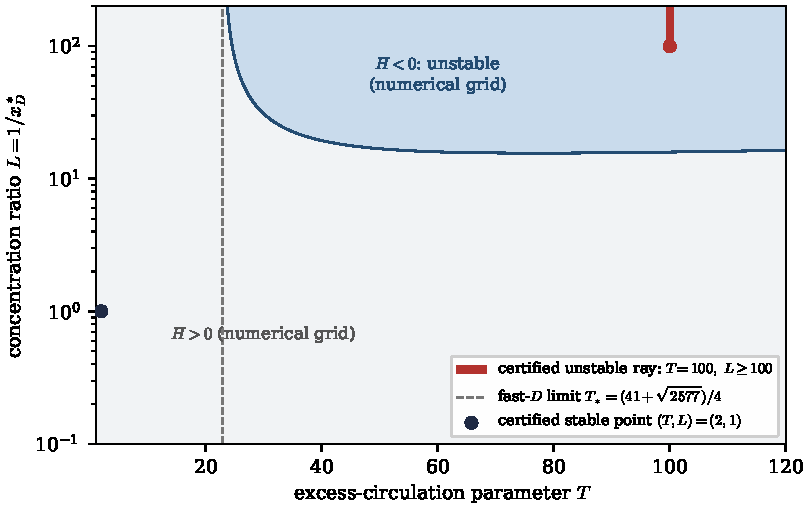
\includegraphics[width=0.78\linewidth]{figures/parameter_region.pdf}
\caption{Sign of the Hurwitz determinant $H(T,L)$ of the family Jacobian $J_0(T,L)$ for $s=1$ and $\xs=(1,1,1,1/L)$. The shaded region and the contour are numerical evaluations of the exact polynomial on a grid, not interval enclosures. The thick vertical segment is part of the certified unstable ray $T=100$, $L\ge100$ (Theorem~\ref{thm:ray}); the dot at $(2,1)$ is the certified stable point (Proposition~\ref{prop:stable}); the dashed line is the large-$L$ threshold $T_*$ (Proposition~\ref{prop:threshold}). The source, its $25$ children and their certificates are the same at every point of the figure. The figure does not cover independent perturbations of the six rate constants; for those see Theorem~\ref{thm:robust}.}
\label{fig:region}
\end{figure}

\subsection{Mechanism: a fast-\texorpdfstring{$D$}{D} Schur reduction}\label{sec:mechanism}

The threshold $T_*$ has a transparent origin. In $J_0(T,L)$ the fourth column carries the factor $L=1/x_D^*$: when $D$ is scarce, its concentration relaxes fast. Eliminating $D$ by the Schur complement with respect to the $(4,4)$ entry gives the reduced $3\times3$ matrix
\[
J_{\mathrm{red}}(T)=J_0^{(3)}-J_0^{(3,4)}\bigl(J_0^{(4,4)}\bigr)^{-1}J_0^{(4,3)} ,
\]
in which $L$ cancels exactly, with characteristic polynomial $z^3+c_1z^2+c_2z+c_3$,
\[
c_1=\frac{14T+32}{T+4},\qquad c_2=\frac{112T}{T+4},\qquad c_3=\frac{64T^2}{T+4},\qquad
c_1c_2-c_3=\frac{32T\,(-2T^2+41T+112)}{(T+4)^2}.
\]
The cubic Hurwitz determinant $c_1c_2-c_3$ changes sign exactly at $T_*$, and it is the factor of the $L^3$ coefficient~\eqref{eq:leading} of $H$. The instability is thus a whole-network fast/slow feedback: a large circulation $v_0=v_2=T$ relative to the return flux $v_3=1$, combined with a fast $D$ pool. The reduced matrix is not the child matrix of any three-species source, so the three-species localization theorem (Proposition~\ref{prop:species}) does not apply to it, and none of the $25$ children, each of which selects at most one consuming reaction per species, records the combination of $r_0$ and $r_3$ through $D$ and of $r_1$ and $r_2$ through $C$ at the common flux.

\section{Robustness and an open-reactor completion}\label{sec:robust}

\begin{theorem}[Rate-space robustness]\label{thm:robust}
Let $k^*=(10000,4,100,10000,99,2)$. There is an open neighbourhood $U$ of $k^*$ in $\R^6_{>0}$ and a smooth map $k\mapsto x(k)\in\R^4_{>0}$ on $U$ with $x(k^*)=\xs$ such that, for every $k\in U$, $x(k)$ is a positive equilibrium of $\mathcal E$ with rate constants $k$ and its Jacobian is Hurwitz-unstable. The source, hence the family of children and their certificates, is unchanged.
\end{theorem}

\begin{proof}
The vector field $F(x,k)=Sv(x,k)$ is polynomial in $(x,k)$ with $F(\xs,k^*)=0$ and $D_xF(\xs,k^*)=J$, and $\det J=64000000\ne0$. The implicit function theorem gives neighbourhoods and a smooth map $x(k)$ with $F(x(k),k)=0$; shrinking $U$ keeps $x(k)$ positive. The matrix $D_xF(x(k),k)$ depends continuously on $k$. Choose a closed disk around the eigenvalue of Proposition~\ref{prop:root}, contained in the open right half-plane and with no eigenvalue of $J$ on its boundary; by continuity of eigenvalues~\cite[App.~D]{HornJohnson2013} it contains an eigenvalue of $D_xF(x(k),k)$ for all $k$ near $k^*$.
\end{proof}

The theorem gives a qualitative open neighbourhood with a moving equilibrium; no quantitative six-dimensional box is claimed. It does not extend to added or reversed reactions or changed integer complexes, which can introduce new children; some of the present certificates lie on the spectral boundary.

\begin{theorem}[Feed and dilution]\label{thm:dilution}
Fix $0<\delta<2$. Let $\mathcal E_\delta$ be the source with twelve reactions consisting of $r_0,r_1,r_2,r_3$ of Table~\ref{tab:source}, four inflows $\varnothing\to X$ for $X\in\{A,B,C,D\}$ with rate constants $(99+\delta,\ \delta,\ \delta,\ 2+\delta/100)$, and four first-order losses $X\to\varnothing$ with rate constant $\delta$. Then $\mathcal E_\delta\in\Rcf$, the point $\xs=(1,1,1,1/100)$ is a positive equilibrium of $\mathcal E_\delta$ with the original rate constants on $r_0,\dots,r_3$, its Jacobian is $J-\delta I$ and is Hurwitz-unstable, and $\mathcal E_\delta$ has no D-unstable core.
\end{theorem}

\begin{proof}
The completed vector field is $F_\delta(x)=F(x)+\delta\xs-\delta x$, because the new inflows equal the old ones plus $\delta\xs$ and the losses contribute $-\delta x$. Hence $F_\delta(\xs)=F(\xs)=0$ and $DF_\delta(\xs)=J-\delta I$. By Proposition~\ref{prop:root}, $J$ has an eigenvalue $\lambda$ with $\Real\lambda\ge2$, so $J-\delta I$ has the eigenvalue $\lambda-\delta$ with $\Real(\lambda-\delta)\ge2-\delta>0$. The losses have reactant molecularity one and no products, and the inflows have no reactants, so $\mathcal E_\delta\in\Rcf$. The absence of D-unstable cores is Lemma~\ref{lem:transport}.
\end{proof}

\begin{lemma}[Child transport under added outflows]\label{lem:transport}
Every child-selection matrix of $\mathcal E_\delta$ is D-nonunstable.
\end{lemma}

\begin{proof}
Let $(I,f)$ be a child selection of $\mathcal E_\delta$. Inflows cannot be selected. Let $O\subseteq I$ be the species assigned to their own loss reaction $X\to\varnothing$, whose stoichiometric column is $-e_X$. The remaining species $I\setminus O$ are assigned reactions of $\mathcal E$ injectively, so $(I\setminus O,f|_{I\setminus O})$ is a child selection of $\mathcal E$. Ordering $O$ first, the child matrix has the block form
\[
C_f=\begin{pmatrix}-I_O&*\\0&C_{\mathrm{old}}\end{pmatrix},
\]
where $C_{\mathrm{old}}$ is the child matrix of $(I\setminus O,f|_{I\setminus O})$ in $\mathcal E$ and the zero block records that a loss column vanishes outside its own species. For any positive diagonal $D=\diag(D_O,D')$, $C_fD$ is block upper triangular with diagonal blocks $-D_O$ and $C_{\mathrm{old}}D'$, so its spectrum is the union of the negative numbers $-d_X$ and the spectrum of $C_{\mathrm{old}}D'$, which lies in the closed left half-plane by Theorem~\ref{thm:children}. Empty blocks cause no exception.
\end{proof}

In flow-reactor form, $F_\delta(x)=S_{\mathrm{act}}v_{\mathrm{act}}(x)+\delta(c_{\mathrm{feed}}-x)$ with feed concentrations $c_{\mathrm{feed}}=(99/\delta+1,\ 1,\ 1,\ 2/\delta+1/100)$; for $\delta=1$ these are $(100,1,1,201/100)$. The extension addresses feeding and washout only; it does not address atom balance or thermodynamic consistency of the internal reactions (Section~\ref{sec:mass}).

\section{Sharpness of the reactant order and species minimality}\label{sec:sharp}

\begin{theorem}[At most one reactant molecule]\label{thm:R1}
Let $(Y,P)$ be a finite source in which every reaction has reactant molecularity at most one, with any positive rate constants. Then every positive equilibrium of~\eqref{eq:mass} has a Hurwitz-nonunstable Jacobian. Catalysts and inflows are allowed.
\end{theorem}

\begin{proof}
A reaction of molecularity zero has constant rate; a reaction of molecularity one has the unique reactant $X_i$ with $Y_{ij}=1$ and rate $k_jx_i$. Hence $F(x)=b+Jx$ with $b=\sum_{\text{inflows}}k_jP_{\cdot j}\ge0$ and $J_{\cdot i}=\sum_{j:\,Y_{ij}=1}k_jS_{\cdot j}$. For $l\ne i$ and $Y_{ij}=1$ we have $Y_{lj}=0$, so $S_{lj}=P_{lj}\ge0$: $J$ is a Metzler matrix. At a positive equilibrium $\xs$, $J\xs=-b\le0$. Put $M=\diag(\xs)^{-1}J\diag(\xs)$; then $M$ is Metzler with row sums $(M\mathbf 1)_i=-b_i/x^*_i\le0$. If $Mz=\lambda z$ with $z\ne0$, choose $i$ with $|z_i|=\max_j|z_j|>0$. Taking the real part of $\lambda|z_i|^2=\sum_jM_{ij}z_j\bar z_i$,
\[
\Real(\lambda)\,|z_i|^2=M_{ii}|z_i|^2+\sum_{j\ne i}M_{ij}\Real(z_j\bar z_i)\le\Bigl(\sum_jM_{ij}\Bigr)|z_i|^2\le0 ,
\]
using $M_{ij}\ge0$ and $\Real(z_j\bar z_i)\le|z_i|^2$ for $j\ne i$. Hence $\Real\lambda\le0$, and $J$ is similar to $M$.
\end{proof}

Thus in the class with reactant molecularity at most one there is no instability at all, and localization holds vacuously; reactant molecularity two is the least for which Theorem~\ref{thm:main} can occur. The argument is the classical maximum-component estimate for Metzler matrices with nonpositive row sums~\cite{BermanPlemmons1994}.

\begin{proposition}[Four species is minimal]\label{prop:species}
Let $(Y,P)$ be a source with at most three species and let $R$ be any reactivity positive exactly on the reactant incidences, in particular the mass-action reactivity~\eqref{eq:J} at any positive equilibrium. If every child-selection matrix of $(Y,P)$ is D-nonunstable, then $SR$ is D-nonunstable, and in particular Hurwitz-nonunstable. Hence four species is the least number of species for which an unstable equilibrium without D-unstable cores exists, in mass action or in any parameter-rich kinetics.
\end{proposition}

\begin{proof}
For exactly three species this is the three-species localization theorem of~\cite{ParameterRich2026}, formalized as \lean{fin_three_noDUnstableChild_implies_jacobian_dNonUnstable}: under the hypothesis on the children, the cubic Routh--Hurwitz determinant of $SR\diag(d)$ is nonnegative for every positive $d$, because it is preserved under positive mixtures of the columns within each species' reaction fibre. A source with fewer species is padded with inert species, that is, zero rows in $Y$ and $P$. Inert species are reactants of no reaction, so the child selections are unchanged, and the padded Jacobian is the original one bordered by zero rows and columns, which adds only zero eigenvalues. The mass-action reactivity is positive exactly on the reactant incidences by~\eqref{eq:J}.
\end{proof}

\begin{remark}[What is not minimal]
A source on four species whose active stoichiometric columns have rank four needs at least five reactions to have a positive stationary flux, which is only the elementary lower bound $m\ge5$. Whether six reactions, or product molecularity nine, can be reduced is not settled here.
\end{remark}

\section{Scope, physical reading and use}\label{sec:scope}

\subsection{Mass balance}\label{sec:mass}

\begin{proposition}[No positive mass vector]\label{prop:mass}
There is no $m\in\R^4_{>0}$ with $m^{\mathsf T}S_{\cdot j}=0$ for $j=0,1,2,3$. Moreover, appending product-only waste species of nonnegative mass to $r_2$ and $r_3$ cannot repair this.
\end{proposition}

\begin{proof}
Conservation across $r_2\colon2C\to D$ gives $m_D=2m_C$, and across $r_3\colon2D\to A+4B+4C$ gives $m_A+4m_B+4m_C=2m_D$, hence $m_A+4m_B=0$, impossible for positive masses. With waste products the two constraints become $m_D\le2m_C$ and $m_A+4m_B+4m_C\le2m_D$, hence $m_A+4m_B\le0$, still impossible.
\end{proof}

Any atom-resolved realization therefore needs an additional material input to $r_3$ (or a changed retained source). A chemostatted fuel species can keep the effective rate quadratic in the retained variables while making the full reactant complex larger than two molecules, and inserting intermediates can create new children. Neither operation is supplied by Theorem~\ref{thm:main}, and the species $A,\dots,D$ are abstract labels, not assigned metabolites. The theorem is about mass-action kinetics on a source, which is exactly the object the conjecture is about.

\subsection{Units}\label{sec:units}

The displayed rate constants are dimensionless. For a concentration scale $C_0$ and a time scale $\tau_0$, put $x_{\mathrm{phys}}=C_0\hat x$ and $t_{\mathrm{phys}}=\tau_0\hat t$; a reaction of reactant molecularity $\mu$ then has
\[
k_{\mathrm{phys}}=\frac{\hat k}{\tau_0\,C_0^{\mu-1}} ,
\]
so the four active second-order constants scale as $1/(\tau_0C_0)$, the two zeroth-order inflows as $C_0/\tau_0$, and a dilution rate as $1/\tau_0$. For example, $C_0=1\,\mathrm{mM}$ and $\tau_0=1\,\mathrm{s}$ give concentrations $(1,1,1,0.01)\,\mathrm{mM}$, second-order constants $(10000,4,100,10000)\,\mathrm{mM^{-1}s^{-1}}$ and inflows $99$ and $2\,\mathrm{mM\,s^{-1}}$. This is a unit conversion, not a calibration: the flux ratio $T=100$, the concentration separation $L=100$ and the resulting stiffness are dimensionless and remain. The event-rate convention for $2C\to D$ and $2D\to\cdots$ is $kx^2$; a stochastic simulator with an unordered-pair propensity must convert separately.

\subsection{A local numerical illustration}\label{sec:local}

Figure~\ref{fig:local} integrates~\eqref{eq:mass} from the initial state $\xs+\varepsilon\,\Real w$, where $w$ is a numerical eigenvector of the unstable eigenvalue $\lambda\approx2.99974676+15.68952573\,i$ normalized to unit maximum modulus and $\varepsilon=10^{-7}$, with a stiff Radau method (relative tolerance $10^{-10}$, absolute tolerance $10^{-13}$) on $\hat t\in[0,0.8]$. The maximal deviation from the linear prediction $\varepsilon\Real(e^{\lambda t}w)$, relative to the maximal linear deviation, is about $6\times10^{-5}$. The local $e$-folding time is $1/\Real\lambda\approx0.3334$ and the rotation period $2\pi/\Imag\lambda\approx0.4005$ in dimensionless time; multiply by $\tau_0$ for physical times. The latter is not a sustained oscillation period, and nothing about the long-time behaviour is asserted.

\begin{figure}[ht]
\centering
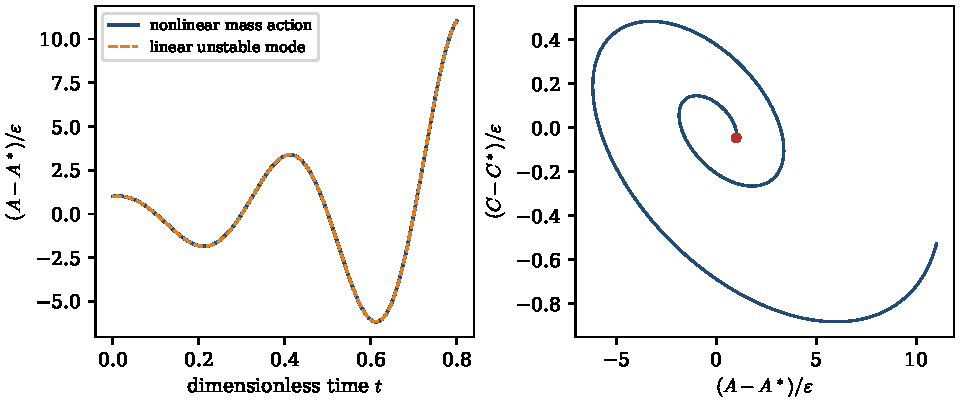
\includegraphics[width=0.9\linewidth]{figures/local_dynamics.pdf}
\caption{Short-time departure from the equilibrium $\xs$ of Table~\ref{tab:source} for a perturbation of size $\varepsilon=10^{-7}$ along the real part of the unstable eigenvector. Left: the $A$ coordinate of the nonlinear solution and of the linear unstable mode. Right: projection to the $(A,C)$ plane; the dot marks the initial state. Numerical illustration only: no periodic orbit, boundedness or persistence is claimed.}
\label{fig:local}
\end{figure}

\subsection{Use as a benchmark}\label{sec:benchmark}

The network is a small exact regression example for software and theorems that infer stability from structure. On $\mathcal E$ with the data of Table~\ref{tab:source} a correct pipeline reports: a positive, exactly stationary state; no D-unstable child and no D-unstable core; an unstable complex eigenpair of the operating-state Jacobian; and therefore that the absence of a D-core does not certify stability of that operating state. Every number is an integer or the rational $1/100$, so the check can be done in exact arithmetic. The supplementary material provides the source, rates, state, flux, characteristic polynomial and the $25$ child certificates in machine-readable form.

For the study of autocatalytic organization, the result separates layers that are sometimes conflated: structural self-sustainment (RAF sets~\cite{HordijkSteel2004}, autocatalytic cores~\cite{BlokhuisLacosteNghe2020}), kinetic feasibility of a positive flux, thermodynamic feasibility, and dynamic stability of an operating state. Theorem~\ref{thm:main} exhibits a failure of one particular structural-to-dynamic implication under low-order mass action; it is not a general failure of structural analysis and it proves no persistence or inheritance statement.

\section{Formal verification and reproducibility}\label{sec:formal}

The statements on the critical path of Theorem~\ref{thm:main}, Corollary~\ref{cor:refutation} and the exact algebra of Section~\ref{sec:family} are verified in Lean~4~\cite{Lean4} with Mathlib~\cite{Mathlib}, compiled with warnings treated as errors and no unproved placeholders, against the frozen toolchain \lean{leanprover/lean4:v4.30.0}. The development lives in \lean{proofs/DUnstableCores/Elementary/} of the accompanying repository and imports the source-network, child-selection, D-scaling and mass-action interfaces of the companion developments~\cite{ParameterRich2026,KineticOrder2026}.

\subsection{What the formal statements say}

A source is a \lean{SourceNetwork} with natural-number reactant and product matrices. A \lean{ClassicalMassActionInstance} of a source carries positive concentrations, positive rate constants, a reactivity, and the \emph{derivative formula} as data: for every reaction $r$ and species $s$,
\[
\text{\texttt{reactivity.value r s}} \;=\; Y_{sr}\cdot\bigl(k_r\cdot\textstyle\prod_ix_i^{Y_{ir}}\bigr)/x_s ,
\]
which is~\eqref{eq:J}. \lean{ClassicalStationary} states $\sum_rS_{sr}\,k_r\prod_ix_i^{Y_{ir}}=0$ for every species; it is proved for the reconstructed monomial rates, not assumed. A \lean{ChildSelection} is a finite set of species with an injective assignment to reactions satisfying the reactant incidence, \lean{realMatrix} is its child matrix, \lean{DNonUnstable} is Definition~\ref{def:spectral}(c) with right scaling, and \lean{IsDUnstableCore} is a D-unstable child minimal under restriction. The two public declarations are, in ASCII rendering,
\begin{verbatim}
theorem elementary_resolution :
  exists Q : SourceNetwork (Fin 4) (Fin 6),
    (forall r, sum s, Q.reactant s r <= 2) and
    (forall s r, Q.reactant s r * Q.product s r = 0) and
    exists M : ClassicalMassActionInstance Q,
      ClassicalStationary M and
      HurwitzUnstable (Q.jacobian M.reactivity) and
      (forall k : ChildSelection Q, DNonUnstable k.realMatrix) and
      not (exists k : ChildSelection Q, IsDUnstableCore k)

theorem reactantBimolecular_core_necessity_false :
  not (forall Q : SourceNetwork (Fin 4) (Fin 6),
    (forall r, sum s, Q.reactant s r <= 2) ->
    forall M : ClassicalMassActionInstance Q, ClassicalStationary M ->
      HurwitzUnstable (Q.jacobian M.reactivity) ->
      exists k : ChildSelection Q, IsDUnstableCore k)
\end{verbatim}
in the namespace \lean{DUnstableCores}. \lean{HurwitzUnstable} asserts an eigenpair with an eigenvalue of positive real part, produced from the root of Proposition~\ref{prop:root} through the characteristic polynomial. The second declaration is the negation of (N$_{\Ract}$) at four species and six reactions; it need not restate catalyst-freedom since the witness of the first already has it.

\subsection{Module map and receipts}

Table~\ref{tab:lean} maps the claims of the paper to Lean modules. The verification receipts record exit code zero, warnings as errors, and axiom reports containing only \lean{propext}, \lean{Classical.choice} and \lean{Quot.sound}; no \lean{sorryAx}, no native computation oracle and no unchecked certificate emitter enters the proofs. The scalar certificates of the $25$ patterns are proved by kernel-checked ring identities and \lean{positivity}, followed by an explicit finite case split; the emitter that produced their text is not trusted.

\begin{table}[ht]
\centering\footnotesize
\begin{tabular}{@{}>{\raggedright\arraybackslash}p{0.27\linewidth}>{\raggedright\arraybackslash}p{0.30\linewidth}>{\raggedright\arraybackslash}p{0.37\linewidth}@{}}
\toprule
Claim & Module & Main declarations\\
\midrule
Literal source, $\Ract$, catalyst-free, positive mass action, stationarity, Jacobian~\eqref{eq:jac} & \lean{ElementarySource.lean} & \lean{elementarySource_R2}, \lean{elementarySource_CF}, \lean{elementaryMassAction_stationary}, \lean{elementaryMassAction_jacobian}\\
\addlinespace
Lemma~\ref{lem:quartic}; Proposition~\ref{prop:root} & \lean{QuarticSpectral.lean} & \lean{elementaryQuartic_no_rhp}, \lean{elementary_exact_quartic_unstable_root}, \lean{elementary_matrix_unstable}\\
\addlinespace
Exact $4\times4$ characteristic coefficients & \lean{FinFourPolynomial.lean} & \lean{elementary_charpoly_fin4}\\
\addlinespace
All $25$ padded patterns D-nonunstable (Remark~\ref{rem:padding}) & \lean{ElementaryPatterns.lean} & \lean{elementary_all_patterns}\\
\addlinespace
Every literal child maps to a pattern; spectral embedding & \lean{ElementaryEmbedding.lean} & \lean{elementaryChildChoice_patterns}, \lean{elementarySource_all_children}\\
\addlinespace
Theorem~\ref{thm:main}, Corollary~\ref{cor:refutation} & \lean{Resolution.lean} & \lean{elementary_resolution}, \lean{reactantBimolecular_core_necessity_false}\\
\addlinespace
Proposition~\ref{prop:cone}, Proposition~\ref{prop:reconstruct} & \lean{ElementaryFluxFamily.lean} & \lean{elementary_positive_stationary_flux_complete}, \lean{elementaryFamilyFlux_reconstruct}\\
\addlinespace
Coefficients~\eqref{eq:famcoeff}; identity~\eqref{eq:Hu}; data of Proposition~\ref{prop:stable} & \lean{ElementaryParameterPolynomial.lean} & \lean{elementary_family_charpoly}, \lean{elementary_fast_D_delta_negative}, \lean{elementary_same_source_control}\\
\addlinespace
Real part at least $2$ (used in Theorem~\ref{thm:dilution}) & \lean{ElementarySpectralMargin.lean} & \lean{elementary_root_real_part_ge_two}\\
\addlinespace
Three-species localization (Proposition~\ref{prop:species}) & \lean{CubicSourceFoldDim3.lean} & \lean{fin_three_noDUnstableChild_implies_jacobian_dNonUnstable}\\
\bottomrule
\end{tabular}
\caption{Scientific claims and the Lean modules that verify them.}
\label{tab:lean}
\end{table}

The root receipt for \lean{Resolution.lean} authenticates both public declarations and its twenty local dependency modules. The SHA-256 of the root source and of the frozen Lake manifest are
\begin{center}\small
\lean{802c322dcae9a9feda0993572cbc98fcebf9a86e592d620949acf16497853fad}\\
\lean{a8df0b606ec258561c226df89856884be433c19b49fb0a27335d69bb2b6e9fac}
\end{center}
The three post-proof leaves have source hashes beginning \lean{b81303f9}, \lean{9413a7a1} and \lean{82ee9f49}; the pattern and embedding modules begin \lean{a3f474c9} and \lean{c8bff145}. Full hashes, build commands and a sequential replay program are in the reproducibility archive accompanying the repository.

\subsection{Conventional statements}

The following are proved in this paper by ordinary mathematics and are not separately formalized: Lemma~\ref{lem:restriction} and the four-maximal-child compression of Section~\ref{sec:children} (the formal development covers all $25$ children directly); Lemma~\ref{lem:converse} and Lemma~\ref{lem:imag}, hence the spectral conclusions of Theorem~\ref{thm:ray}, Proposition~\ref{prop:stable} and Proposition~\ref{prop:threshold} beyond the formally checked coefficient identities; the Schur reduction of Section~\ref{sec:mechanism}; Theorem~\ref{thm:robust}; Theorem~\ref{thm:dilution} and Lemma~\ref{lem:transport} (which use the formal margin and the formal child exclusion); Theorem~\ref{thm:R1}; the inert-padding step of Proposition~\ref{prop:species}; Proposition~\ref{prop:mass}; Remark~\ref{rem:routh}. All printed constants were re-derived in exact rational arithmetic while drafting; the figures are numerical illustrations and are not evidence for any statement.

\section{Open problems}\label{sec:open}

\begin{question}[Two-sided bimolecular networks]
Does D-unstable-core necessity hold for classical mass-action networks in which every reaction has at most two reactant molecules and at most two product molecules ($\Rpp$), with or without catalysts? The nine-molecule product complex of $r_3$ is the only obstacle to placing $\mathcal E$ in this class, and Proposition~\ref{prop:mass} shows that a conservative realization would in any case need additional inputs.
\end{question}

\begin{question}[Minimal size]
What are the least numbers of reactions and the least maximal product molecularity of a reactant-bimolecular mass-action network with an unstable positive equilibrium and no D-unstable core? Four species is minimal (Proposition~\ref{prop:species}) and at least five reactions are needed; six and nine are upper bounds.
\end{question}

\begin{question}[Nonlinear dynamics]
Does the unstable complex pair of $\mathcal E$ arise through a Hopf bifurcation along the family of Section~\ref{sec:family}, and does the network sustain a periodic orbit? The present results concern the linearization only.
\end{question}

\begin{question}[Corrected localization]
Which finite structural data, beyond the child lattice, suffice to localize complex-pair instabilities of low-order mass-action networks? Section~\ref{sec:mechanism} suggests that fast/slow Schur reductions weighted by a feasible stationary flux are the relevant objects.
\end{question}

\bibliographystyle{plain}
\bibliography{refs}

\end{document}
